\documentclass[a4paper, 12pt]{article}
%%%%%%%%%%%%%%%%%%%%%%%%%%%%%%%%%%%%%%%%%%%%%%%%%%%%%%%%%%%%%%%%%%%
    %Pacotes carregados%
%%%%%%%%%%%%%%%%%%%%%%%%%%%%%%%%%%%%%%%%%%%%%%%%%%%%%%%%%%%%%%%%%%%    
\usepackage[utf8]{inputenc}         %Permite acentuação
\usepackage[brazilian]{babel}       %Identifica erro gramatical e mudança de linguagem
\usepackage{amsmath}
\usepackage{graphicx}               %Importação de imagem
\usepackage{cite}                   %Pacote de citações
\usepackage{makeidx}                %Pacote para gerar sumário
\usepackage{enumerate}              %Pacote para utilizar o ambiente enumerate
\usepackage{indentfirst}            %Pacote que corrige o espaço dos parágrafos
\usepackage{setspace}               %Pacote de espaçamento entre linhas
\usepackage{enumitem}               %Pacote de ambiente itemize
\usepackage{hyperref}               %Pacote de gerenciamento de hiperlinks
\usepackage{url}                    %Pacote de gerenciamento de urls
\usepackage{colortbl}               %Pacote que permite o uso de cores nas tabelas
\usepackage{booktabs}               %Pacote para estilizar a coluna de tabelas
\usepackage{siunitx}                %Utilização de unidades do SI
\usepackage{placeins}               %Permite usar FloatBarrier pra delimitar até onde uma figura pode aparecer
\usepackage{float}
\usepackage{listings}               %Pacote que permite adicionar códigos ao texto
\usepackage{amssymb}
%\usepackage[alf]{abntex2cite}      %Referências em ABNT... BUG
\usepackage[left=3.00cm, right=2.00cm, top=3.00cm, bottom=2.00cm]{geometry}                                                     %Margem padrão ABNT

\let\Oldsection\section
\renewcommand{\section}{\FloatBarrier\Oldsection} %Figuras de uma seção não podem aparecer em outra seção

\let\Oldsubsection\subsection
\renewcommand{\subsection}{\FloatBarrier\Oldsubsection} %Figuras de uma subseção não podem aparecer em outra subseção

\let\Oldsubsubsection\subsubsection
\renewcommand{\subsubsection}{\FloatBarrier\Oldsubsubsection} %Figuras de uma subsubseção não podem aparecer em outra subsubseção

\sisetup{per-mode=symbol} %usa / ao invés de ^-1 em unidades do tipo V/A
\renewcommand{\subsection}{\FloatBarrier\Oldsubsection} %Figuras de uma subseção não podem aparecer em outra subseção


\hypersetup{colorlinks = true, linkcolor=black, urlcolor = blue, citecolor = black}

\lstdefinelanguage{AMPL}{keywords={set,param,var,arc,integer,minimize,maximize,subject,to,node,sum,in,Current,complements,integer,solve_result_num,IN,contains,less,suffix,INOUT,default,logical,sum,Infinity,dimen,max,symbolic
,Initial,div,min,table,LOCAL,else,option,then,OUT,environ,setof ,union,all,exists,shell_exitcodeuntil,binary,forall,solve_exitcodewhile ,by,if,solve_messagewithin,check,in,solve_result
},sensitive=true,comment=[l]{\#}}

\lstset{frame=tb,
  language=AMPL,
  aboveskip=3mm,
  belowskip=3mm,
  showstringspaces=false,
  columns=flexible,
  basicstyle={\ttfamily},
  numbers=none,
  numberstyle=\tiny\color{gray},
  keywordstyle=\bfseries,
  commentstyle=\textit,
  stringstyle=\color{mauve},
  breaklines=true,
  breakatwhitespace=true,
  tabsize=3
}                %Arquivo de configuração do trabalho

\begin{document}
    \onehalfspacing                 %Para um espaçamento de 1,5 padrão ABNT
    %============================================================================
%======================= PRIMEIRA FOLHA INTERNA  ============================
%============================================================================
\begin{titlepage}
    \vspace*{2.0cm}
    \begin{center}
    \large{Lucas Zenichi Terada}
    \end{center}
    
    
    \vspace*{4.8cm}
    
    \begin{center}
    {\sc \Large  Reconfiguração das redes de distribuição de energia elétrica operando em diferentes níveis de demanda}
    \end{center}
    
    
    \vspace*{3.25cm}
    
    
    \null \vfill
    
    \begin{center}
    Campinas\\2018
    \end{center}
\end{titlepage}
%=============================================================================
%============================= FOLHA DE ROSTO ================================
%=============================================================================

\begin{center}
\large Universidade Estadual de Campinas\\
Faculdade de Engenharia Elétrica e de Computação
\end{center}

\vspace*{1.0cm}
\begin{center}
\large Lucas Zenichi Terada
\end{center}

    
\vspace*{1.3cm}
    
\begin{center}
    {\sc Reconfiguração das redes de distribuição de energia elétrica operando em diferentes níveis de demanda}
\end{center}
    
\vspace*{0.5cm}

    
\vspace*{1.0cm}
    
\begin{flushright}
\begin{minipage}{11.0cm}
Projeto de iniciação científica financiada pela Fundação de Amparo e Pesquisa do Estado de São Paulo. 
    
\vspace*{0.5cm}
    
\vspace*{1.0cm}
Orientador: Marcos Julio Rider Flores
    
\end{minipage}
\end{flushright}
    
\null \vfill
\begin{minipage}{7cm}
\small
Este exemplar corresponde ao relatório parcial do projeto de iniciação científica.    
\rule{6.9cm}{0.2mm} \hfill 
\end{minipage}
    
\null \vfill
\begin{center}
    Campinas\\2018
\end{center}
\thispagestyle{empty}
\newpage         %Capa do projeto de iniciação científica
    {\Large\textbf{Resumo das atividades}}
\par
{\Large\textbf{Resumo}}


\newpage
\listoffigures                  %Inserção da lista de figuras
\newpage                        
\listoftables                   %Inserção da lista de tabelas
\newpage

{\large\textbf{Nomenclatura}}

\newpage


        %Elementos pré-textuais
    \tableofcontents                %Sumário
    \newpage
    \section{Introdução}

Os sistemas de distribuição de energia elétrica (SDEE) são planejados como redes malhadas interconectadas.
Entretanto, operam como com uma topologia radial a fim da facilitar a coordenação da proteção e reduzir a corrente de curto circuito dos SDEE.
Para obter uma topologia radial existem chaves de interconexões em pontos estratégicos do sistema.
Desse modo, a topologia inicial pode ser modificada pela operação das chaves para transferir as demandas entre os diferentes alimentadores e, assim, é possível determinar uma nova topologia com outro ponto de operação, contudo deve continuar sendo uma topologia radial.

O problema de reconfiguração de sistemas de distribuição (RSD) consiste na abertura e/ou fechamento das chaves com o objetivo de melhorar um índice de desempenho. 
A reconfiguração ótima é uma importante ferramenta para aumentar a confiabilidade de um SDEE, especialmente quando a automação avançada e tecnologias de redes inteligentes (smartgrids) tornam-se mais importante e mais acessível às concessionarias de distribuição.






    \section{Objetivos}
    \section{Metodologia}

\subsection{Introdução a Linguagem de Programação Matemática}

\subsection{Hipóteses e definições da formulação do problema}

\begin{figure}[H]
    \centering
    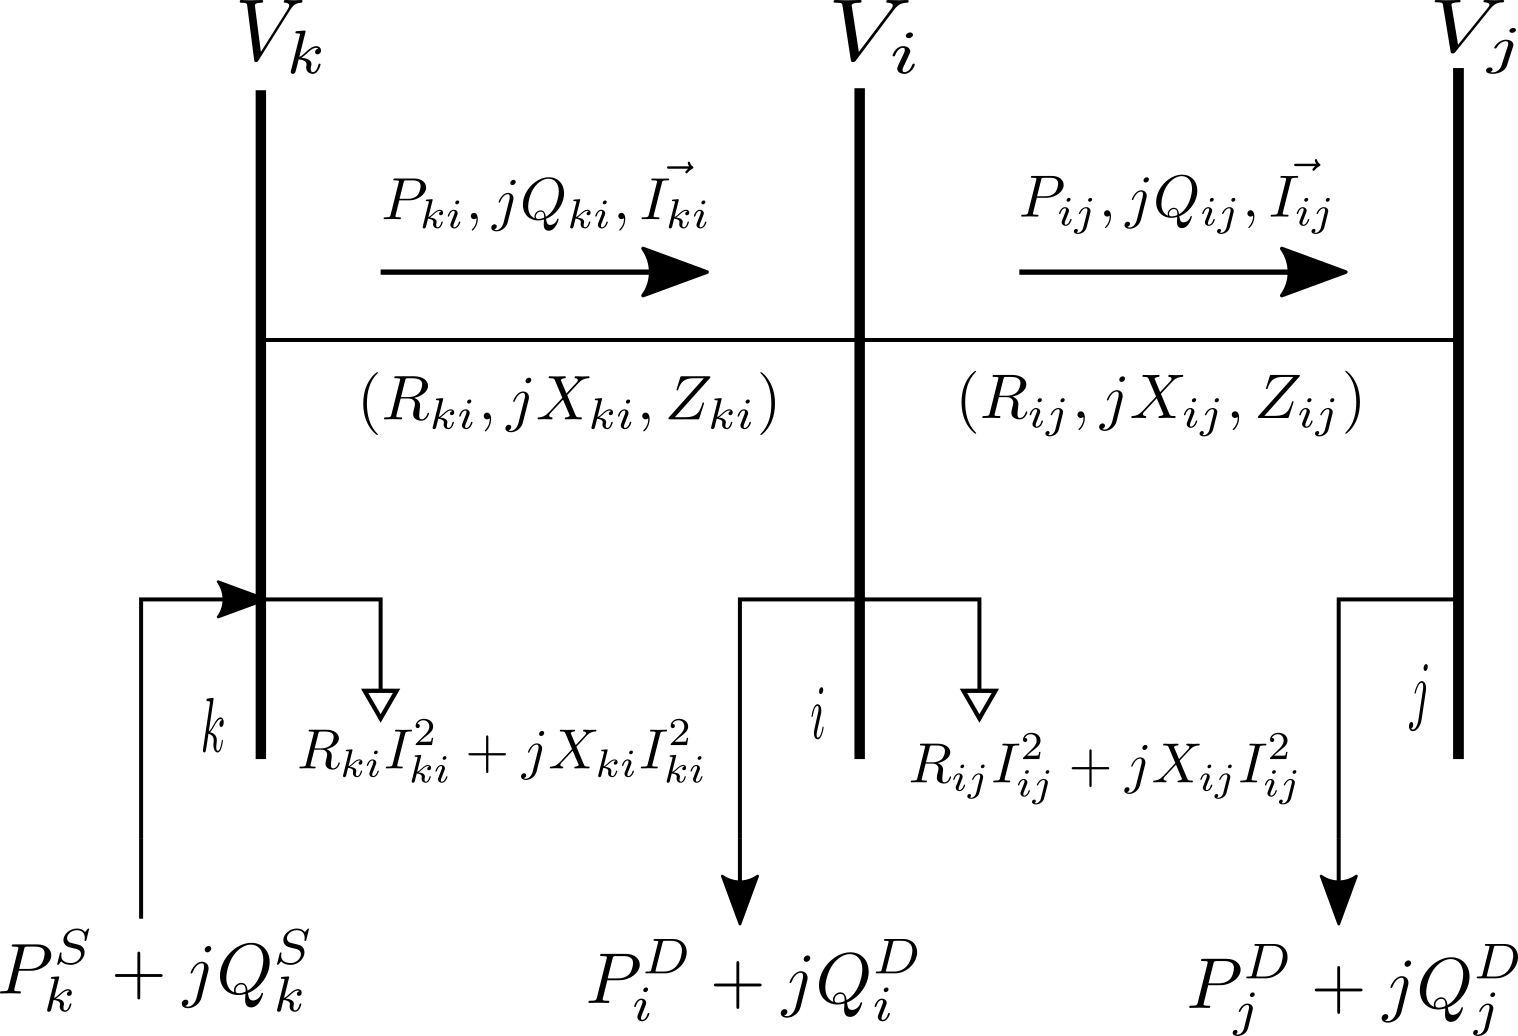
\includegraphics[scale = 1.2]{01_img/diagrama_nos.png}
    \caption{Sistema de distribuição radial}
    \label{fig:SDR}

\end{figure}

Hipóteses adotadas:
Visando representar o funcionamento em regime permanente de um sistema de distribuição de energia, são feitas as seguintes hipóteses (comumente usadas nas formulações de varredura de fluxo de carga \cite{ShirmohammadiANetworks} e mostradas na figura \ref{fig:SDR}.

\begin{itemize}
    \item As demandas nas cargas na rede de distribuição são representadas como potência ativa e reativas contantes;
    
    \item O sistema é balanceado e representado pelo seu equivalente monofásico;
    
    \item As perdas de potência ativa e reativa no circuito \textit{ij} estão concentradas no nó \textit{i}.
    
    \item As chaves são representadas como circuito curtos de impedância nula.
\end{itemize}
    \section{Restrições do problema}


    \subsection{Balanço de potência}

\begin{figure}[H]
    \centering
    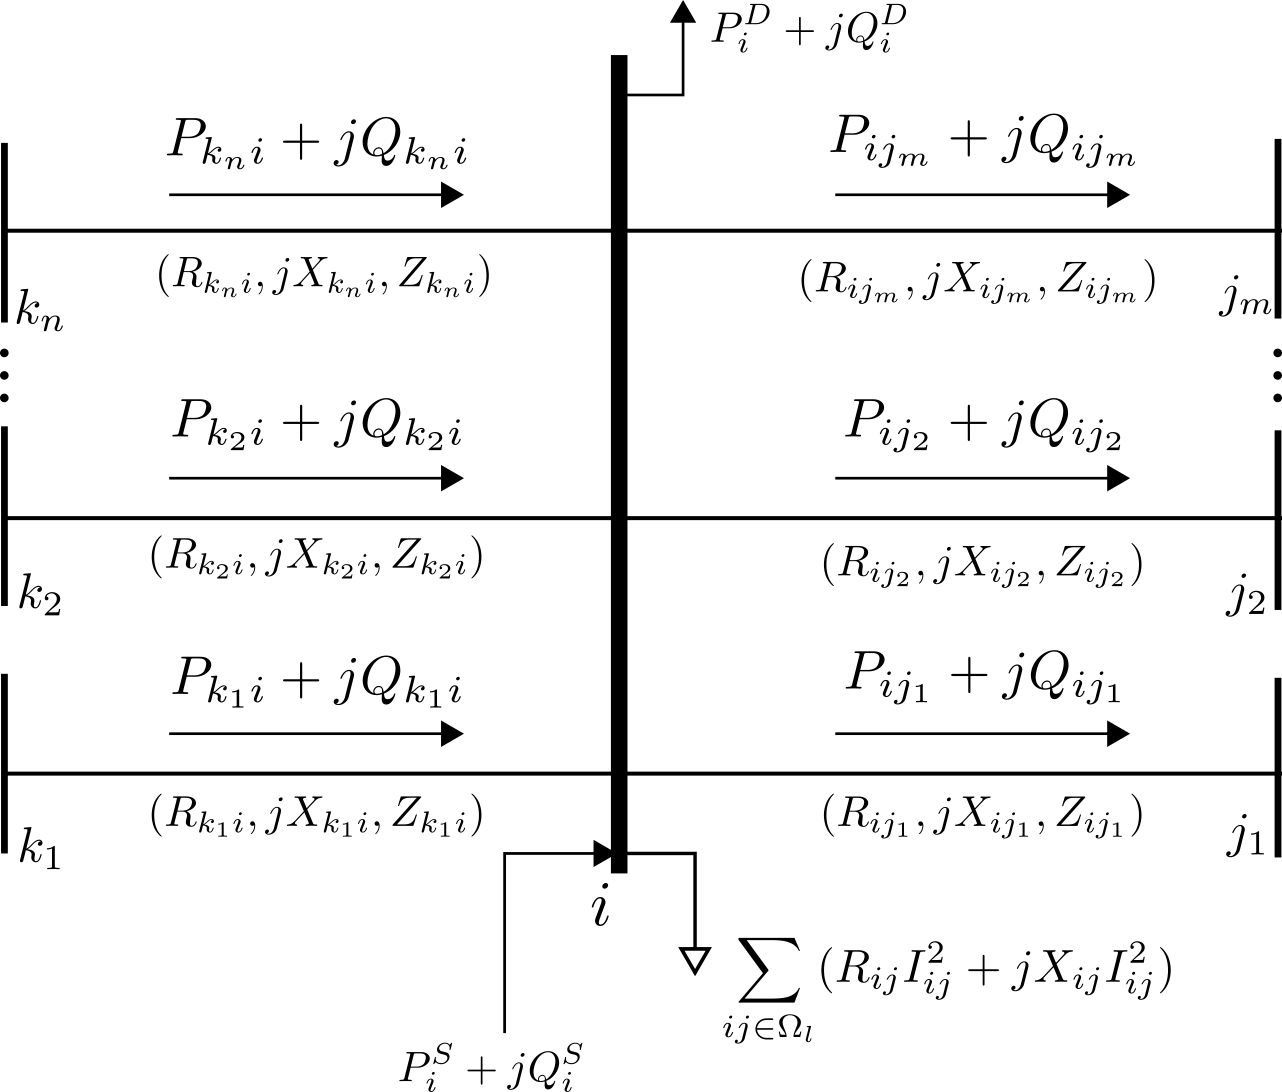
\includegraphics[scale = 1.4]{01_img/diagrama_potencia.png}
    \caption{Exemplo de um diagrama de balanço de potência entre nós de um sistema de distribuição de energia elétrica}
    \label{fig:balanco_pot}
\end{figure}

A figura~\ref{fig:balanco_pot} representa a forma expandida da figura~\ref{fig:SDR}, para melhor compreensão do problema de balanço de potência, onde $m$ e $n$ representam um número qualquer de nós ligados ao nó $i$. 
Para isso considere que nos parâmetros e variáveis que representam um ramo, o primeiro subíndice representa o nó de partida e o segundo subíndice o nó de chegada (exemplo: $P_{12}$ representa o fluxo de potência ativa que vai do nó 1 para o nó 2).

Seja $P_{i}^{D}$ e $Q_{i}^{D}$ potência ativa e reativa demandada no nó i respectivamente e $P_{i}^{S}$ e $Q_{i}^{S}$ potência ativa e reativa gerada no nó i respectivamente, têm-se que:

\begin{equation*}
    \sum_{ki\in\Omega_{l}}P_{ki} - \sum_{ij\in\Omega_{l}}(P_{ij} + R_{ij}I_{ij}^{2}) + P_{i}^{S} = P_{i}^{D}\quad\forall i \in\Omega_{b}
\end{equation*}

\begin{equation*}
    \sum_{ki\in\Omega_{l}}Q_{ki} - \sum_{ij\in\Omega_{l}}(Q_{ij} + X_{ij}I_{ij}^{2}) + Q_{i}^{S} = Q_{i}^{D}\quad\forall i \in\Omega_{b}
\end{equation*}

Tal que, $\Omega_{l}$ é o conjunto de circuitos e $\Omega_{b}$ é o conjunto de nós.
É possível mudar a variável \textit{k} pela variável \textit{j}, uma vez que ambas pertencem ao conjunto $\Omega_{l}$ e os somatórios envolvendo-as estão desconectadas, desse modo:

\begin{equation}
    \sum_{ji\in\Omega_{l}}P_{ji} - \sum_{ij\in\Omega_{l}}(P_{ij} + R_{ij}I_{ij}^{2}) + P_{i}^{S} = P_{i}^{D}\quad\forall i \in\Omega_{b}\label{eq:fluxo_pot_ativa}  
\end{equation}


\begin{equation}
    \sum_{ji\in\Omega_{l}}Q_{ji} - \sum_{ij\in\Omega_{l}}(Q_{ij} + X_{ij}I_{ij}^{2}) + Q_{i}^{S} = P_{i}^{D}\quad\forall i \in\Omega_{b}\label{eq:fluxo_pot_reativa}
\end{equation}

O sistema de equações não lineares em \ref{eq:fluxo_pot_ativa} e \ref{eq:fluxo_pot_reativa} representam a operação em regime permanente de uma rede elétrica radial e são frequentemente utilizados no método de varredura de fluxo de carga \cite{ShirmohammadiANetworks} e \cite{DeliveryNewNetworks}

    \subsection{Queda de tensão entre nós}


Formulação do Problema de Fluxo de Carga para redes elétricas radiais:

Da figura \ref{fig:SDR}, a queda de tensão do circuito é definida pela equação \ref{eq:queda_tensao}.

\begin{equation}
    \Vec{V}_{i} - \Vec{V}_{j} = I_{ij}(R_{ij} + jX_{ij})\quad\forall ij \in \Omega_{l}
    \label{eq:queda_tensao}
\end{equation}

Em que $\Omega_{l}$ é o conjunto de circuitos. %OBSERVAÇÃO: Explicar mais sobre o conjunto de circuitos
Através da fórmula para o cálculo da potência aparente, $I_{ij}$ pode ser calculado usando a equação \ref{eq:corrente_ramo}.

\begin{equation}
    I_{ij} = \left(\frac{P_{ij} + jQ_{ij}}{\Vec{Vj}}\right)^{*}\quad\forall ij \in \Omega_{l}
    \label{eq:corrente_ramo}
\end{equation}

%OBSERVAÇÃO: Explicar o uso da tensão Vj e as potências (Considerou-se que as perdas ao longo do ramo ij estão concentradas no nó i, por isso a potência que passa ao longo do ramo é a potência Sij que é igual a potência drenada do nó j

Substituindo $I_{}ij$ da equação \ref{eq:corrente_ramo} na equação \ref{eq:queda_tensao} obtém-se a equação \ref{eq:queda_tensao_pot} que define a queda de tensão em função das potências e impedâncias do circuito.

Seja $(P_{ij} + jQ_{ij})^{*} = (P_{ij} - jQ_{ij})$ logo:

\begin{equation}
    (\Vec{V}_{i} - \Vec{V}_{j})\Vec{V}_{j}^{*} = (P_{ij} - jQ_{ij})(R_{ij} + jX_{ij}) \quad\forall ij \in \Omega_{l}
    \label{eq:queda_tensao_pot}
\end{equation}

Considerando que $\Vec{V}_{i} = V_{i}\angle{\theta_{i}}$, $\Vec{V}_{j} = V_{j}\angle{\theta_{j}}$ e $\theta_{ij} = \theta_{i} - \theta_{j}$, tal que  $V_{i}$ e $V_{j}$ representam as magnitudes da tensão em seus respectivos nós bem como $\theta_{i}$ e $\theta_{j}$ representam seus ângulos.
Dessa forma a equação \ref{eq:queda_tensao_pot} pode ser escrita decompondo a fase de suas exponenciais, como mostra a equação \ref{eq:queda_tensao_sencos}.

\begin{equation}
    V_{i}V_{j}[cos\theta_{ij} + jsen\theta_{ij}] - V_{j}^{2} = (P_{ij} - jQ_{ij})(R_{ij} + jX_{ij}) \quad\forall ij \in \Omega_{l}
    \label{eq:queda_tensao_sencos}
\end{equation}

Identificando as partes real e imaginária na equação \ref{eq:queda_tensao_sencos}, obtém-se:

\begin{equation}
    V_{i}V_{j}cos\theta_{ij} = V_{j}^{2} + (R_{ij}P_{ij} + X_{ij}Q_{ij})\quad\forall ij \in \Omega_{l}
    \label{eq:queda_tensao_real}
\end{equation}

\begin{equation}
    V_{i}V_{j}sen\theta_{ij} = X_{ij}P_{ij} - R_{ij}Q_{ij}\quad\forall ij \in \Omega_{l}
    \label{eq:queda_tensao_imaginaria}
\end{equation}

Usando a fórmula da trigonometria, que é a relação básica entre o seno e o cosseno, $sen^{2}(\theta_{ij}) + cos^{2}(\theta_{ij}) = 1$, e somando os quadrados das equações \ref{eq:queda_tensao_real} e \ref{eq:queda_tensao_imaginaria}, obtém-se:

\begin{equation}
    V_{i}^{2} - 2(R_{ij}P_{ij} + X_{ij}Q_{ij}) - Z_{ij}^{2}I_{ij}^{2} - V_{j}^{2} = 0\quad\forall ij \in \Omega_{l}
    \label{eq:queda_tensao_restricao}
\end{equation}

Note que a equação \ref{eq:queda_tensao_restricao} não depende da diferença angular entre as tensões, e é possível obter a magnitude da tensão do nó ($V_j$) em termos da magnitude inicial ($V_i$), o fluxo de potência ativa ($P_{ij}$), o fluxo de potência reativa ($Q_{ij}$), a magnitude do fluxo de corrente ($I_{ij}$) e os parâmetros elétricos do ramo \textit{ij}.



    \subsection{Fluxo de corrente em um ramo}

Na equação de queda de tensão, a magnitude do fluxo de corrente $I_{ij}$ é mostrado na equação \ref{eq:corrente_magnitude} calculado a partir do produto com seu complexo conjugado.

\begin{equation}
    I_{ij}^{2} = \frac{P_{ij}^{2}+Q_{ij}^{2}}{V_{j}^{2}}\quad\forall ij \in \Omega_{l}
    \label{eq:corrente_magnitude}
\end{equation}

    \subsection{Restrições operativas do sistema}

Como visto as equações \ref{eq:fluxo_pot_ativa}, \ref{eq:fluxo_pot_reativa}, \ref{eq:queda_tensao_restricao} e \ref{eq:corrente_magnitude}
são restrições cujas variáveis $V_{i}$ e $I_{ij}$ estão sempre na forma quadrática, por isso é possível fazer uma substituição de variável a fim de tornar mais simples o problema, tal que:

\begin{align*}
    I_{ij}^{sqr} = I_{ij}^{2} \text{ e } V_{i}^{sqr} = V_{i}^{2} 
\end{align*}

Assim é possível determinar as restrições operativas para o funcionamento da SDEE.

%Buscar referências quanto a 

\subsubsection{Limites de tensão}

Em um sistema de distribuição de energia elétrica é preciso garantir que a tensão em um nó deva estar dentro de uma faixa de operação determinada por norma, por isso uma restrição fundamental para o problema é a restrição de limites de tensão em um nó, determinada pela seguinte equação:

\begin{equation}
    \underline{V}^{2} \leq V_{i}^{sqr} \leq \overline{V}^{2}\qquad i \in\Omega_{b}
\end{equation}

Onde $\underline{V}$ e $\overline{V}$ representam os limites inferiores e superiores de tensão, respectivamente, que uma rede pode possuir.

\subsubsection{Limite de corrente}

Assim como as tensões, o fluxo de corrente também deve ser limitado para não comprometer o SDEE.
Assim a equação que descreve a restrição é:

\begin{equation}
    0 \leq I_{ij}^{sqr} \leq \overline{I}_{ij}^{2} \qquad ij\in\Omega_{l} 
\end{equation}

\subsubsection{Chaves presentes no sistema}

Para reconfiguração do SDEE, existem chaves ao longo da rede que podem ser modificadas de modo a garantir a operação desejada.
Considere as seguintes restrições:

\begin{figure}[h]
    \centering
    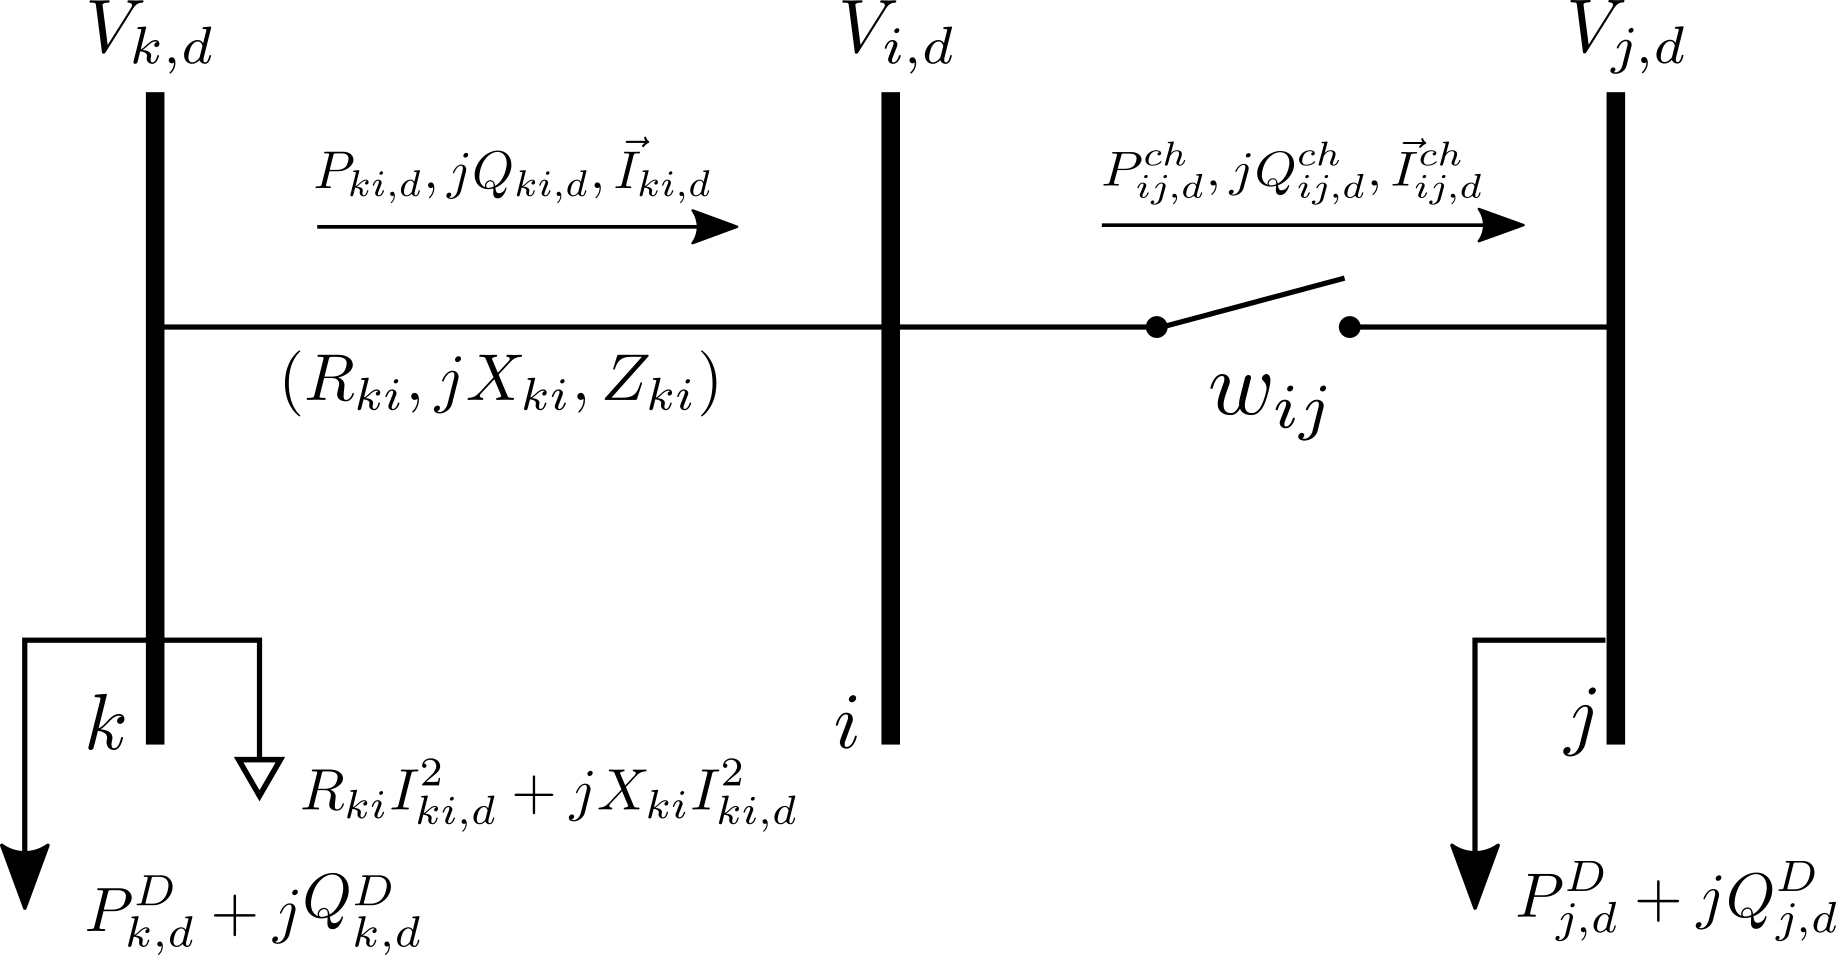
\includegraphics[scale = 1.5]{01_img/diagrama_chaves.png}
    \caption{Modelo de uma Cl conectada entre dois nós}
    \label{fig:diagrama_chave}
\end{figure}
    
\begin{itemize}
    \item Balanço de potência
\end{itemize}
    Com base na figura \ref{fig:diagrama_chave} faz-se necessário reformular as equações de balanço de potência adicionando as variáveis que representam as chaves na modelagem do problema.
    
\begin{equation}
    \sum_{ji\in\Omega_{l}}P_{ji} - \sum_{ij\in\Omega_{l}}(P_{ij} + R_{ij}I_{ij}^{2})+ \sum_{ji\in\Omega_{ch}}P_{ji}^{ch} -\sum_{ij\in\Omega_{ch}}P_{ij}^{ch} + P_{i}^{S} = P_{i}^{D}\quad\forall i \in\Omega_{b}\label{eq:fluxo_pot_ativa_chaves}  
\end{equation}
    
    
\begin{equation}
    \sum_{ji\in\Omega_{l}}Q_{ji} - \sum_{ij\in\Omega_{l}}(Q_{ij} + X_{ij}I_{ij}^{2})+ \sum_{ji\in\Omega_{ch}}Q_{ji}^{ch} -\sum_{ij\in\Omega_{ch}}Q_{ij}^{ch} + Q_{i}^{S} = P_{i}^{D}\quad\forall i \in\Omega_{b}
    \label{eq:fluxo_pot_reativa_chaves}
\end{equation}
    
Onde $\Omega_{ch}$ representa o conjunto de chaves da rede elétrica e $w_{ij}$ é uma variável binária que representa o estado da chave \textit{ij}, se $w_{ij} = 1$ a chave ij está fechada, caso contrário a chave está aberta, ver figura~\ref{fig:diagrama_chave}. $P_{ij}^{ch}$ e $Q_{ij}^{ch}$ representam o fluxo de potência ativa e reativa da chave \textit{ij}.
    
As restrições expressas nas equações \ref{eq:fluxo_pot_ativa_chaves} e \ref{eq:fluxo_pot_reativa_chaves} são uma extensão das equações \ref{eq:fluxo_pot_ativa} e \ref{eq:fluxo_pot_reativa}, considerando a presença de chaves na rede elétrica.
    
Além do balanço de potência outras restrições devem ser estabelecidas devido a presença de chaves, são elas:
    
\begin{itemize}
    \item Diferença de tensões entre dois nós conectadas por uma chave
\end{itemize}

    
A diferença de tensão entre nós, na presença de chaves, deve ser igual a zero, uma vez que, de acordo com as hipóteses adotadas, a impedância da chaves é representada como uma impedância nula.
Sendo assim, usando as variável binária $w_{ij}$ é possível equacionar a restrição da seguinte forma:
    
\begin{equation}
    -(\overline{V}^{2} - \underline{V}^{2})(1-w_{ij}) \leq V_{i}^{sqr} - V_{j}^{sqr} \leq (\overline{V}^{2} - \underline{V}^{2})(1-w_{ij})\qquad ij\in\Omega_{ch}        
\end{equation}
    
Note que se $w_{ij}$ for igual a 1 (chave fechada), a diferença entre as tensões no nó $i$ e nó $j$ será igual a zero, o que condiz a hipótese adotada.
\begin{itemize}
   \item Fluxo de potência na chave
\end{itemize} 
    
O fluxo de potência na chave é determinada pelas equações abaixo.
    
\begin{equation}
    -(\overline{V}\,\overline{I}_{ij}^{ch})w_{ij} \leq P_{ij}^{ch} \leq (\overline{V}\,\overline{I}_{ij}^{ch})w_{ij}\qquad ij\in\Omega_{ch}   
\end{equation}
    
    
\begin{equation}
    -(\overline{V}\,\overline{I}_{ij}^{ch})w_{ij} \leq Q_{ij}^{ch} \leq (\overline{V}\,\overline{I}_{ij}^{ch})w_{ij}\qquad ij\in\Omega_{ch}   
\end{equation}
    
Note que se a variável $w_{ij}$ for igual a 0 (chave aberta) o fluxo de potência na chave é igual a zero o que condiz com a proposta do elemento de circuito na rede, quando igual a 1 as restrições representam o fluxo máximo de potência ativa e reativa permitida na chave quando está energizada.

\subsubsection{Restrição de radialidade}

A representação de um SDEE é feita através de nós e circuitos. Fazendo analogia com a teoria de grafos, um SDEE pode ser considerado como um grafo formado por n arcos e m nós.
Da teoria de grafos, uma árvore é um grafo conexo sem ciclos, assim é possível comparar a topologia radial de um SDEE com uma árvore.
Como mostrado em \cite{Bazaraa1990LinearFlows}, a árvore de um grafo é um sub-grafo com ($m-1$) arcos.

Assim, pode-se dizer que a topologia de um SDEE com $n_{b}$ nós é radial se satisfaz as duas seguintes condições: Condição 1: a solução deve apresentar ($n_{b}$) circuitos; e Condição 2: a solução deve gerar uma topologia conexa. Note que a restrição de radialidade tem que ser formada pelas condições 1 e 2.
Somente a condição 1 não garante a radialidade do SDEE. O problema de RSD cumpre com as seguintes características: 1) apenas uma única subestação existente no SDEE (nó da subestação); 2) todos os outros nós são nós de carga; 3) a primeira lei de kirchhoff, deve ser cumprida, e 4) o objetivo é encontrar a melhor topologia radial. 
A condição 1 é satisfeita pela seguinte restrição:

\begin{equation}
    |\Omega_{l}| + \sum_{ij\in\Omega_{ch}}w_{ij} = |\Omega_{b}| - 1
    \label{eq:radialidade}
\end{equation}

Em que $|\Omega|$ é um operador que calcula o número de elementos do conjunto $\Omega$.

Uma solução que satisfaz a restrição de balanço de potência (primeira Lei de Kirchhoff) tem de fornecer a demanda de potência em cada nó de carga. De modo que existe um caminho entre a subestação e os nós de carga. Portanto, cada nó está ligado com a subestação, formando um grafo conexo, o que comprova a Condição 2. 
Assim, quando as restrições de balanço de potência são combinadas com a Condição 1, cada nó de carga está ligada por um único caminho com a subestação, isto é, o SDEE é conexo, sem malhas.

\begin{figure}[H]
    \centering
    
\includegraphics[scale = 1]{01_img/restricao_fail.png}
    \caption{Exemplo de rede não radial que obedece a equação \ref{eq:radialidade}}
    \label{fig:radialidade_wrong}
\end{figure}

Observe que a figura \ref{fig:radialidade_wrong}, embora respeite a equação \ref{eq:radialidade} (5 ramos para 6 nós), não é uma topologia radial. Isso pode acontecer se levar somente em consideração a equação \ref{eq:radialidade}.

\begin{figure}[H]
    \centering
    
\includegraphics[scale =0.8]{01_img/restricao_radialidade.png}
    \caption{Exemplo de rede radial que obedece a equação \ref{eq:radialidade}}
    \label{fig:radialidade_right}
\end{figure}

Observe agora a figura \ref{fig:radialidade_right}, note que ela é uma topologia radial, como dito anteriormente é necessário duas condições para garantir tal configuração, como no problema já existem equações que garantem a primeira Lei de Kirchhoff, a topologia final será radial. 
Observe que todos os nós estão interligados, direto ou indiretamente, com o nó 1 (nó da subestação). 
Isso acontece pois as equações de balanço de potência obrigam que haja fluxo de potência para atender as demandas dos mesmos.

Assim a equação \ref{eq:radialidade} junto com \ref{eq:fluxo_pot_ativa_chaves} e \ref{eq:fluxo_pot_reativa_chaves} fornecem as condições necessárias para e suficientes para garantir uma topologia final radial \cite{Lavorato2012ImposingProblems}.


    \section{Modelo matemático do problema}

Com base nas deduções e hipóteses adotadas anteriormente, o problema de reconfiguração de uma rede elétrica radial pode ser representado utilizando um modelo de programação linear inteiro misto (PNLIM), mostrado a seguir:

\begin{equation*}
    \text{Min} = c^{lss}\sum_{ij\in\Omega_{l}}R_{ij}I_{ij}^{sqr}
\end{equation*}

Sujeito a:

\begin{equation*}
    \sum_{ji\in\Omega_{l}}P_{ji} - \sum_{ij\in\Omega_{l}}(P_{ij} + R_{ij}I_{ij}^{sqr})+ \sum_{ji\in\Omega_{ch}}P_{ji}^{ch} -\sum_{ij\in\Omega_{ch}}P_{ij}^{ch} + P_{i}^{S} = P_{i}^{D}\quad\forall i \in\Omega_{b}  
\end{equation*}
    
\begin{equation*}
    \sum_{ji\in\Omega_{l}}Q_{ji} - \sum_{ij\in\Omega_{l}}(Q_{ij} + X_{ij}I_{ij}^{sqr})+ \sum_{ji\in\Omega_{ch}}Q_{ji}^{ch} -\sum_{ij\in\Omega_{ch}}Q_{ij}^{ch} + Q_{i}^{S} = Q_{i}^{D}\quad\forall i \in\Omega_{b}
\end{equation*}

\begin{equation*}
    V_{i}^{sqr} - 2(R_{ij}P_{ij} + X_{ij}Q_{ij}) - Z_{ij}^{2}I_{ij}^{sqr} - V_{j}^{sqr} = 0\quad\forall ij \in \Omega_{l}
\end{equation*}

\begin{equation*}
    V_{j}^{sqr}I_{ij}^{sqr} = P_{ij}^{2}+Q_{ij}^{2}\quad\forall ij \in \Omega_{l}
\end{equation*}

\begin{equation*}
    -(\overline{V}^{2} - \underline{V}^{2})(1-w_{ij}) \leq V_{i}^{sqr} - V_{j}^{sqr} \leq (\overline{V}^{2} - \underline{V}^{2})(1-w_{ij})\qquad ij\in\Omega_{ch}        
\end{equation*}
    
\begin{equation*}
    -(\overline{V}\,\overline{I}_{ij}^{ch})w_{ij} \leq P_{ij}^{ch} \leq (\overline{V}\,\overline{I}_{ij}^{ch})w_{ij}\qquad ij\in\Omega_{ch}
\end{equation*}
    
    
\begin{equation*}
    -(\overline{V}\,\overline{I}_{ij}^{ch})w_{ij} \leq Q_{ij}^{ch} \leq (\overline{V}\,\overline{I}_{ij}^{ch})w_{ij}\qquad ij\in\Omega_{ch}   
\end{equation*}
    
\begin{equation*}
    |\Omega_{l}| + \sum_{ij\in\Omega_{ch}}w_{ij} = |\Omega_{b}| - 1
\end{equation*}

\begin{equation*}
    \underline{V}^{2} \leq V_{i}^{sqr} \leq \overline{V}^{2}\qquad i \in\Omega_{b}
\end{equation*}

\begin{equation*}
    0 \leq I_{ij}^{sqr} \leq \overline{I}_{ij}^{2} \qquad ij\in\Omega_{l} 
\end{equation*}

\begin{equation*}
    w_{ij}\quad\text{binário}\qquad\forall ij \in\Omega_{ch}
\end{equation*}
    \section{Implementando o PNLIM}

A implementação do problema de programação não linear inteiro misto, obtido da análise física e operativa da rede, no AMPL é dada a partir de 3 arquivos principais.
O arquivo de extensão .mod possui a modelagem do problema com base na formulação algébrica das restrições adequado a linguagem do AMPL. 

\lstinputlisting[language=AMPL,caption=Arquivo que contém o programa que modelo o problema de reconfiguração de sistema de distribuição radial, label={lst:mod_file}]{02_code/PNLIM_RSD.mod}

Os demais arquivos principais de extensão \verb|.dat| e \verb|.run| estão nos anexos, juntamente com arquivos auxiliares.


%\gls{}

    \bibliographystyle{ieeetr}       %Estilo de apresentação da bibliografia
    \bibliography{mendeley_v2}            %Insere referencias ao texto
    
\end{document}
